\chapter{Opis projektnog zadatka}
    \section{Uvod}
		
		Igra \textit{GlobeRunner} zamišljena je kao način da se ljude potakne na istraživanje lokalnih povijesnih i prirodnih znamenitosti. Pri posjetima znamenitostima igrači će se kretati na otvorenom, što je svakako bolja alternativa provođenju vremena u zatvorenom prostoru. Kroz same bitke, odnosno odabir kartica za njih, igrači će bolje upoznati bitne atribute lokalnih znamenitosti kraj kojih često prolaze bez razmišljanja jer će im upravo pažljiv odabir znamenitosti donositi pobjede u bitkama protiv drugih igrača.\par
		
		Platforme sa sličnom vizijom već postoje, jedna od njih je \textit{Geocaching}, Slika \ref{fig:geocaching}. Radi se o igri koja se zasniva na skrivenim spremnicima (eng. \textit{geocaches}) koji sadrže mali dnevnik u koji se posjetitelji zapisuju kada ga pronađu. Igrači u samoj aplikaciji biraju koji spremnik žele pronaći i zatim se upute u potragu. Prilikom pronalaska u spremniku mogu ostaviti i neku sitnicu, ili pak uzeti nešto iz njega, a nakon pronalaska svoje dojmove mogu objaviti na platformi. Razlika u odnosu na igru \textit{GlobeRunner} jest u tome da postoje fizički artefakti koji se skrivaju na proizvoljna mjesta i zatim pronalaze, dok je cilj ove igre sam posjet lokaciji koja treba biti na neki način značajna, povijesno ili pak geografski. Po pitanju nepostojanja fizičkih artefakata, \textit{GlobeRunner} je sličniji igri \textit{Pokémon GO} u kojoj se uz mjesta lokalnih znamenitosti vežu zamišljena bića iz animirane japanske franšize \textit{Pokémon}, zbog čega se pak razlikuje po značenju samih virtualnih artefakata. Sam tijek igre, kroz bitke u kojima se koriste kartice, podsjeća na kolekcionarsku igru \textit{Yu-Gi-Oh!}, no cijela premisa igre u potpunosti je drugačija.
		
		\begin{figure}[H]
			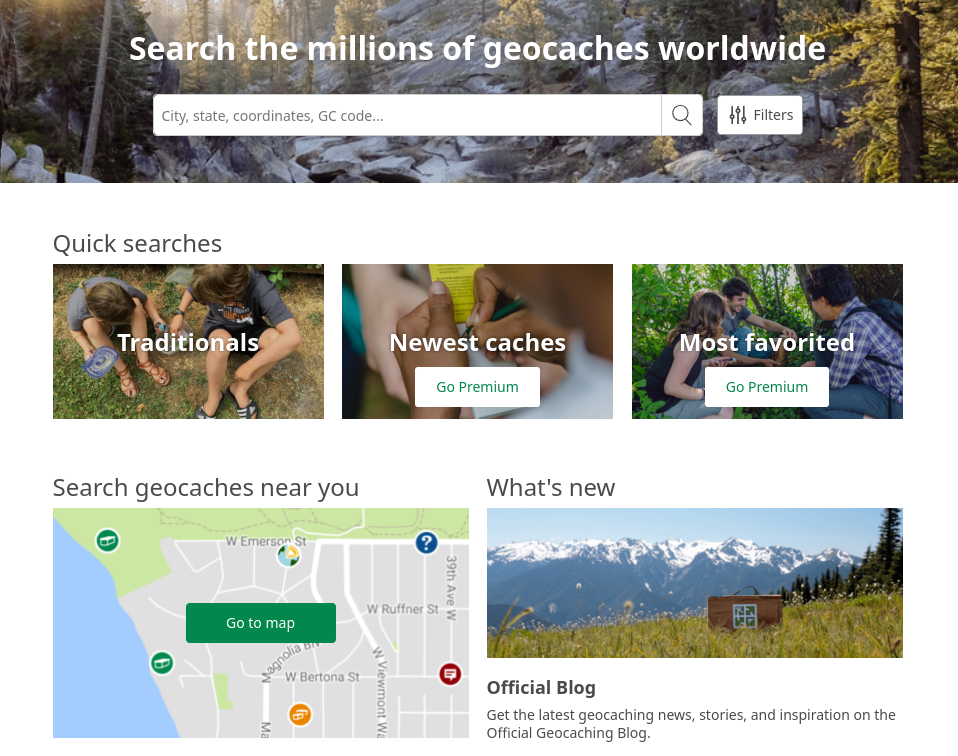
\includegraphics[width=\textwidth]{slike/Uvod/Geocaching.png} 
			\caption{Web sjedište platforme \textit{Geocaching}}
			\label{fig:geocaching}
		\end{figure}
		
		Upravo bi iz navedenih razloga \textit{GlobeRunner} mogao privući igrače koji žele na zabavan način upoznati područja u kojima borave i kojima se kreću, kojeg god uzrasta bili, dok god paze na svoju sigurnost, posebno pri posjeti izazovnijim lokacijama poput planinskih vrhova. Ova aplikacija otvara svoja vrata i onim najznatiželjnijima koji žele poboljšati igru, odnosno predložiti nove lokacije i tako istaknuti njihov značaj.
		
		\section{Cilj i očekivane funkcionalnosti}
		
		Cilj je ovog projekta razviti programsku potporu za web aplikaciju, odnosno igru GlobeRunner, koja će igračima omogućiti prikupljanje kartica koje su vezane uz neke geografske ili povijesne znamenitosti tako što će fizički doći na lokaciju same znamenitosti. Svaka lokacija ima minimalno naziv, opis i fotografiju. Nakon što skupi karticu, igrač ju može koristiti u bitkama protiv drugih igrača u svojoj blizini. Izazov koji očekujemo nakon puštanja aplikacije u pogon jest populacija baze podataka jer je postojanje kartica za skupljanje premisa za privlačenje igrača. Stoga je cilj razvoja programske potpore osigurati i postojanje mogućnosti da igrači doprinesu igri predlaganjem novih kartica, ali i da ti doprinosi budu pregledani i odobreni od strane za to ovlaštenih korisnika - kartografa.

		
		Prilikom pokretanja sustava prikazuje se stranica dobrodošlice za neautentificirane korisnike na kojoj se ukratko predstavlja igra i nude gumbi "Prijavi se", "Postani igrač" i "Postani kartograf".  Prijava postojećeg korisnika vrši se email adresom ili korisničkim imenom i lozinkom, dok su za registraciju novog \underbar{igrača} potrebni sljedeći podatci:
		\begin{packed_item}
		    \item korisničko ime
		    \item fotografija
		    \item lozinka
		    \item email adresa
		\end{packed_item}
		
		Za registraciju \underbar{kartografa} potrebni su i sljedeći podatci:
		\begin{packed_item}
		    \item IBAN računa (za uplatu naknade)
		    \item fotografija osobne iskaznice
		\end{packed_item}
		
		Nakon ispunjavanja obrasca za registraciju, novi igrač treba potvrditi svoju e-mail adresu klikom na dostavljenu poveznicu. Tako potvrđen igrač može krenuti s upotrebom web aplikacije, dok registraciju kartografa naknadno mora odobriti administrator.
		
		\underbar{Igrač} nakon registracije započinje igru s predefiniranim početnim brojem bodova u ELO sustavu (npr. u šahu je 1500). Nakon prijave igrač vidi početnu stranicu koja prikazuje kartu na kojoj su označene lokacije s karticama koje još nije prikupio. Kada se igrač nađe u blizini neskupljenih kartica, ispod karte se pojavi popis kartica u neposrednoj blizini, njih onda može pokušati pokupiti pritiskom na gumb "Pokupi" koji će to dopustiti samo ako je igrač jako blizu kartici. Na početnoj stranici, kao i na ostalima, igrač vidi i izbornik koji mu omogućuje navigaciju kroz web aplikaciju. Sadržaj izbornika je sljedeći:
		
		\begin{packed_item}
		    \item Vlastiti profil
		    \item Globalna statistika
		    \item Igrači u blizini
		\end{packed_item}
		
		Kroz izbornik igrač može pristupiti vlastitom profilu na kojem vidi statistiku svojih borbi i sve karte koje je skupio. U izborniku se također nalazi i poveznica na stranicu "Globalna statistika" koja prikazuje ljestvicu svih igrača sortiranu po ELO bodovnom sustavu, a uz to prikazuje i statistiku svih odigranih bitki i skupljenih kartica u igri. Do stranice koja prikazuje popis drugih igrača u blizini igrač također dolazi preko spomenutog izbornika. Na tom popisu igrač odabire koga će izazvati, a nakon što drugi igrač prihvati izazov, svaki odabire karte s kojima će ići u bitku. Iznad spomenutog popisa igraču se pojave zahtjevi za bitke kada ih drugi igrači izazovu, a on ih onda može prihvatiti ili odbiti. Bitka se provodi usporedbom površina koje razapinju tri kartice koje pojedini igrač odabere, uz napomenu da se površina skalira prosjekom jačina tih triju kartica. Jačina kartice smanjuje se nakon svakog korištenja i to smanjenje vrijedi samo za korisnika koji ju koristi. Nakon svake bitke igračima se ažurira njihov broj bodova shodno ELO sustavu. Ako igrač pređe određeni prag bodova, dodjeljuje mu se status naprednog igrača.
		
		\underbar{Napredni igrač}, uz sve spomenute funkcionalnosti običnog igrača, u svom izborniku ima i opciju "Dodaj lokaciju" koja ga vodi na stranicu za predlaganje nove lokacije, odnosno kartice. Kako bi dodao neku lokaciju, napredni igrač mora biti u njezinoj blizini. U obrazac za dodavanje lokacije mora unijeti sve podatke koje kartica treba imati - naziv, opis i fotografiju. Nakon što predloži novu lokaciju, ona mu postaje vidljiva na njegovoj karti za dodavanje, ali uz naznaku da još nije odobrena.
		
		\underbar{Kartograf} je poseban korisnik aplikacije koji ima ulogu pregledavanja, dopunjavanja i odobravanja predloženih lokacija za popunjavanje baze podataka. Prilikom prijave u sustav kartograf na početnoj stranici vidi kartu na kojoj mu se, ovisno o odabranim filtrima, prikazuju prijedlozi za nove kartice i/ili već odobrene kartice. Zadatak je kartografa da odbaci prijedlog ako već postoji lokacija koja se pokušava dodati. Ako lokacija već ne postoji u bazi, onda kartograf pregledava i uređuje opis, naziv i fotografiju nakon čega karticu može odobriti ili pak označiti da ju treba provjeriti na terenu, pri čemu ju dodaje u listu kartica koje treba provjeriti. Putem izbornika kartograf može pristupiti sljedećim funkcionalnostima:
		
		\begin{packed_item}
		    \item Vlastiti profil
		    \item Provjera na terenu
		\end{packed_item}
		
		Na stranici vlastitog profila kartograf ima uvid u kartice koje je već odobrio. Stranica za provjeru na terenu daje kartografu priliku da iz liste kartica koje treba provjeriti na terenu odabere one koje će on provjeriti. Tako dopunjava svoju listu kartica za obići. Kada označi željeni broj lokacija za provjeru, kartograf klikom na gumb "generiraj rutu" zadaje sustavu problem trgovačkog putnika koji sustav rješava koristeći vanjski servis OSRM te kartografu prikazuje rutu koju treba obići da bi na terenu provjerio sve kartice koje je odabrao.
		
		\underbar{Administrator} ima ulogu nadgledanja korisnika, lokacija i kartografa, a u tu svrhu u svom izborniku ima pristup sljedećim stranicama:
		
		\begin{packed_item}
		    \item Svi korisnici
		    \item Sve kartice
		    \item Odobravanje kartografa
		\end{packed_item}
		
		Na stranici "Svi korisnici" administratoru se prikazuje popis svih korisnika. Za svakog korisnika nudi mu se opcija uređivanja osobnih podataka i opcija isključenja iz igre koje ga vode na pripadne stranice s tim funkcionalnostima. Na stranici "Sve kartice" administratoru je prikazana karta sa svim karticama u igri, a klikom na bilo koju od njih administrator dobiva opciju uređivanja kartice izmjenom bilo kojeg atributa same kartice. "Odobravanje kartografa" je stranica putem koje administrator dobiva uvid u registracije kartografa koje još nisu odobrene. Za svaku od njih nudi mu se opcija da ju odobri.
		
		Uz očekivane funkcionalnosti, identificirali smo i nadogradnje sustava koje bi poboljšale sigurnost, performanse i iskustvo korisnika, a čiji razvoj nije dio ovog projekta. Neke od njih su:
		
		\begin{packed_item}
		    \item Složeniji proces borbe
		    \item Funkcija obnavljanja snage kartice ponovnim skupljanjem
		    \item ...
		\end{packed_item}
		
		\section{Primjeri u \LaTeX u}
		
		\textit{Ovo potpoglavlje izbrisati.}\\

		U nastavku se nalaze različiti primjeri kako koristiti osnovne funkcionalnosti \LaTeX a koje su potrebne za izradu dokumentacije. Za dodatnu pomoć obratiti se asistentu na projektu ili potražiti upute na sljedećim web sjedištima:
		\begin{itemize}
			\item Upute za izradu diplomskog rada u \LaTeX u - \url{https://www.fer.unizg.hr/_download/repository/LaTeX-upute.pdf}
			\item \LaTeX\ projekt - \url{https://www.latex-project.org/help/}
			\item StackExchange za Tex - \url{https://tex.stackexchange.com/}\\
		
		\end{itemize} 	


		
		\noindent \underbar{podcrtani tekst}, \textbf{podebljani tekst}, 	\textit{nagnuti tekst}\\
		\noindent \normalsize primjer \large primjer \Large primjer \LARGE {primjer} \huge {primjer} \Huge primjer \normalsize
				
		\begin{packed_item}
			
			\item  primjer
			\item  primjer
			\item  primjer
			\item[] \begin{packed_enum}
				\item primjer
				\item[] \begin{packed_enum}
					\item[1.a] primjer
					\item[b] primjer
				\end{packed_enum}
				\item primjer
			\end{packed_enum}
			
		\end{packed_item}
		
		\noindent primjer url-a: \url{https://www.fer.unizg.hr/predmet/proinz/projekt}
		
		\noindent posebni znakovi: \# \$ \% \& \{ \} \_ 
		$|$ $<$ $>$ 
		\^{} 
		\~{} 
		$\backslash$ 
		
		
		\begin{longtblr}[
			label=none,
			entry=none
			]{
				width = \textwidth,
				colspec={|X[8,l]|X[8, l]|X[16, l]|}, 
				rowhead = 1,
			} %definicija širine tablice, širine stupaca, poravnanje i broja redaka naslova tablice
			\hline \multicolumn{3}{|c|}{\textbf{naslov unutar tablice}}	 \\ \hline[3pt]
			\SetCell{LightGreen}IDKorisnik & INT	&  	Lorem ipsum dolor sit amet, consectetur adipiscing elit, sed do eiusmod  	\\ \hline
			korisnickoIme	& VARCHAR &   	\\ \hline 
			email & VARCHAR &   \\ \hline 
			ime & VARCHAR	&  		\\ \hline 
			\SetCell{LightBlue} primjer	& VARCHAR &   	\\ \hline 
		\end{longtblr}
		

		\begin{longtblr}[
				caption = {Naslov s referencom izvan tablice},
				entry = {Short Caption},
			]{
				width = \textwidth, 
				colspec = {|X[8,l]|X[8,l]|X[16,l]|}, 
				rowhead = 1,
			}
			\hline
			\SetCell{LightGreen}IDKorisnik & INT	&  	Lorem ipsum dolor sit amet, consectetur adipiscing elit, sed do eiusmod  	\\ \hline
			korisnickoIme	& VARCHAR &   	\\ \hline 
			email & VARCHAR &   \\ \hline 
			ime & VARCHAR	&  		\\ \hline 
			\SetCell{LightBlue} primjer	& VARCHAR &   	\\ \hline 
		\end{longtblr}
	


		
		
		%unos slike
		\begin{figure}[H]
		    \centering
			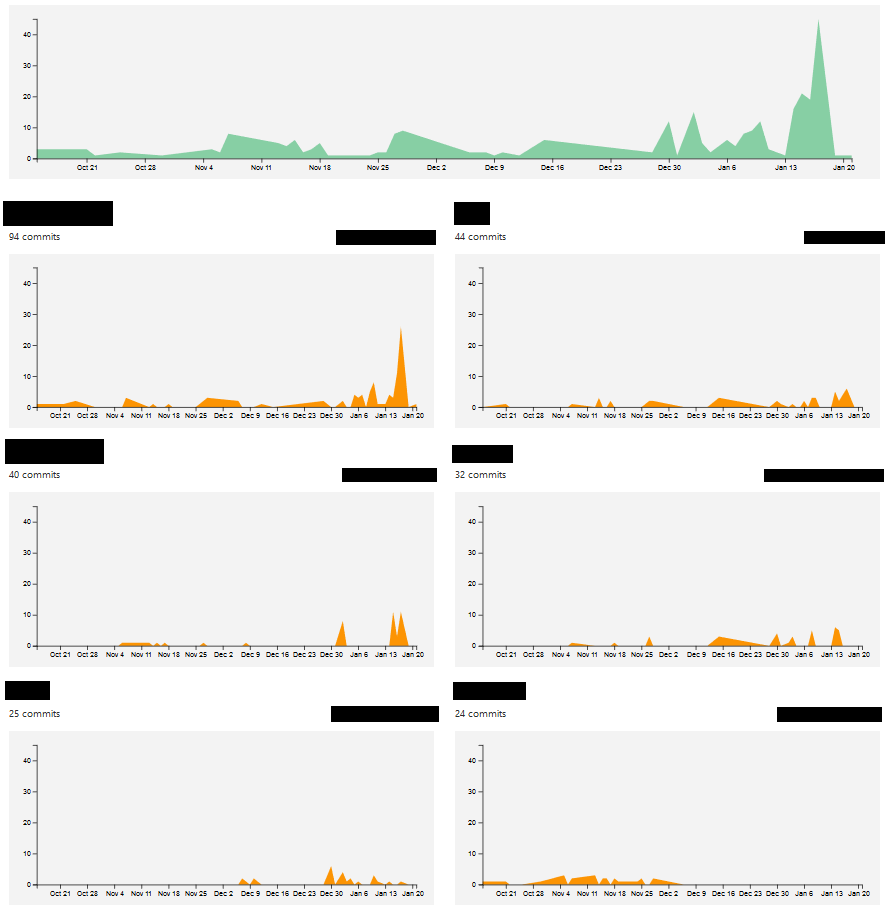
\includegraphics[scale=0.4]{slike/aktivnost.PNG} %veličina slike u odnosu na originalnu datoteku i pozicija slike
			\centering
			\caption{Primjer slike s potpisom}
			\label{fig:promjene}
		\end{figure}
		
		\begin{figure}[H]
			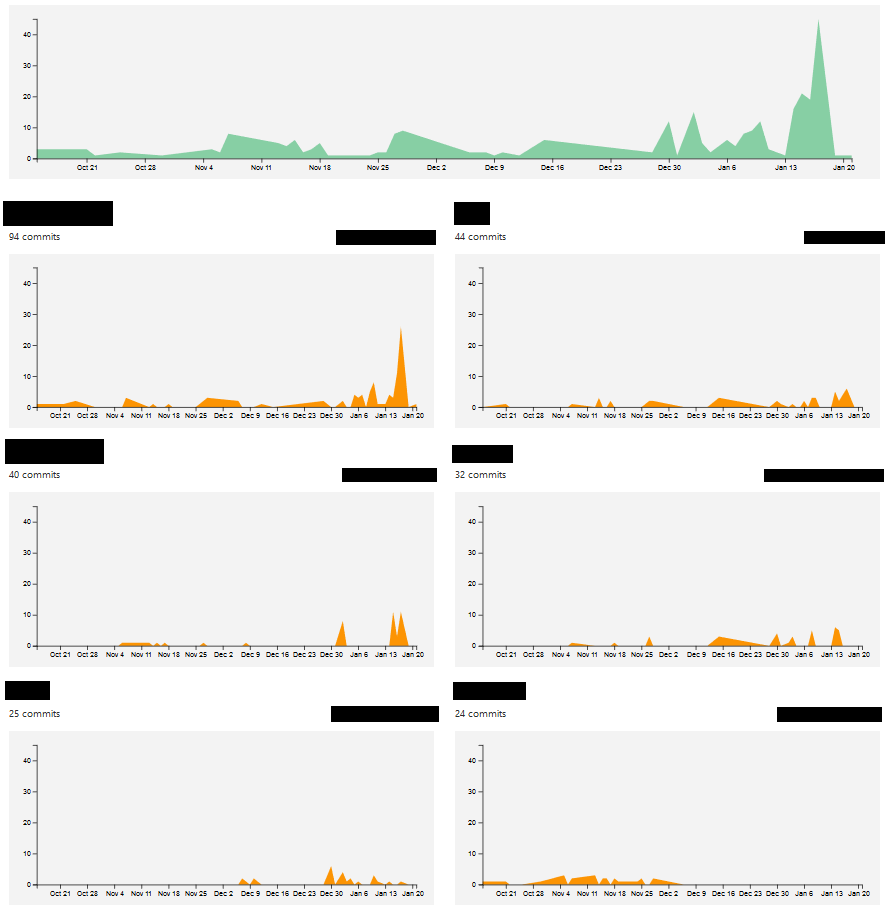
\includegraphics[width=\textwidth]{slike/aktivnost.PNG} %veličina u odnosu na širinu linije
			\caption{Primjer slike s potpisom 2}
			\label{fig:promjene2} %label mora biti drugaciji za svaku sliku
		\end{figure}
		
		Referenciranje slike \ref{fig:promjene2} u tekstu.
		
		\eject
		
	